{
\setbeamertemplate{navigation symbols}{}
\setbeamercolor{background canvas}{bg={black}}
\color{white}
\begin{frame}[plain]
\fontsize{36pt}{36pt}\selectfont
\center
\begin{center}
Refactored Registration Framework
\end{center}

\fontsize{12pt}{12pt}\selectfont
\begin{center}
Insight Software Consortium
\end{center}
\newline
\begin{center}
 PICSL @ University of Pennsylvania 
\end{center}
\newline
\begin{center}
 Brian Avants, Nicholas Tustison, Gang Song, \\ 
Baohua Wu, Michael Stauffer, James C. Gee
\end{center}
\end{frame}
}

\setbeamertemplate{background}{
\includegraphics[width=\paperwidth]{../Art/ITKv4_transparent}}
\begin{frame}
\frametitle{What is registration?}
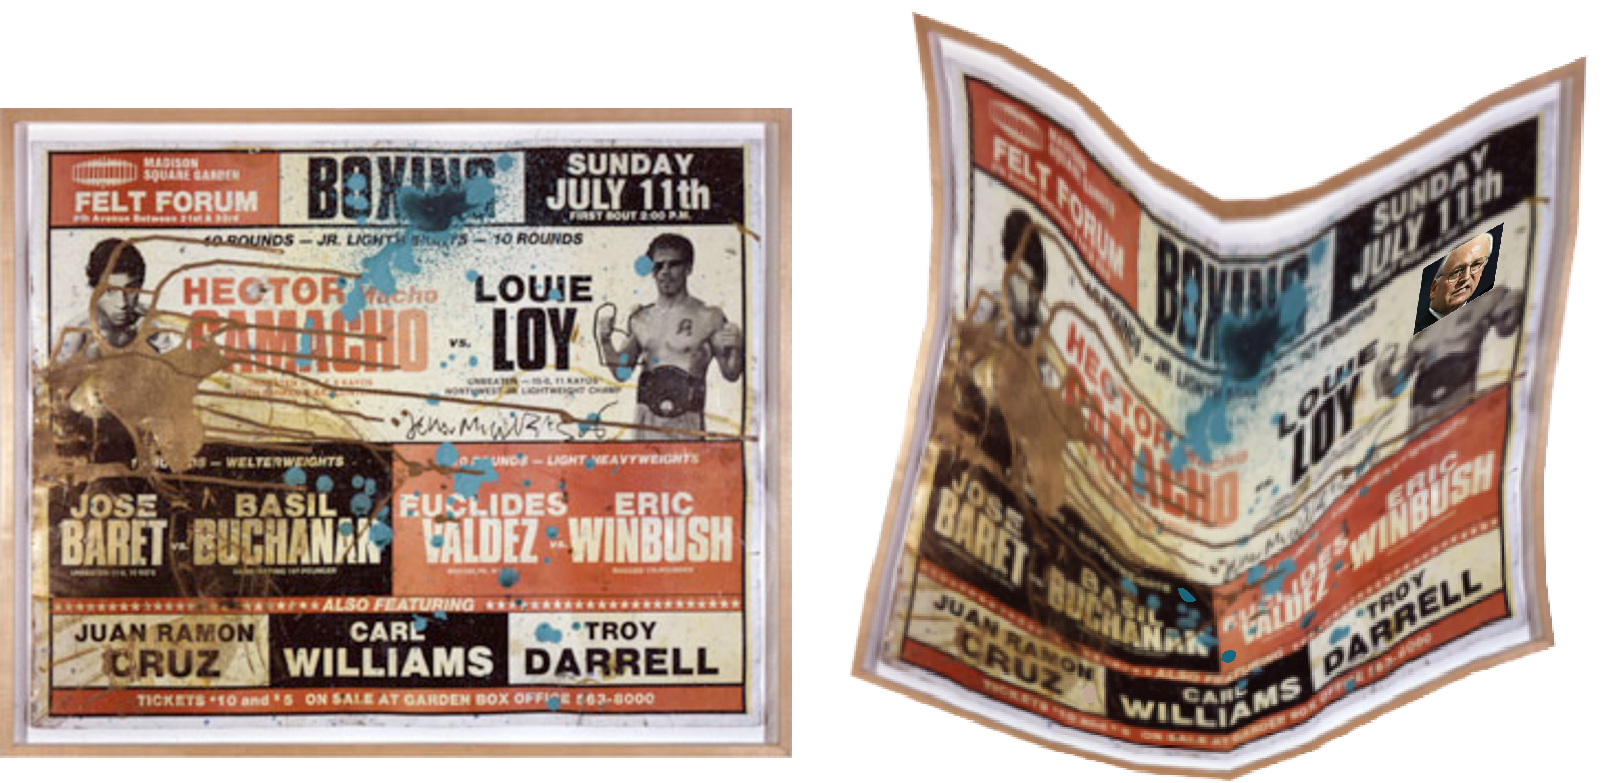
\includegraphics[height=2in]{../Art/RegistrationBasquiatWarp.pdf}
\end{frame}

\begin{frame}
\frametitle{What is registration?}
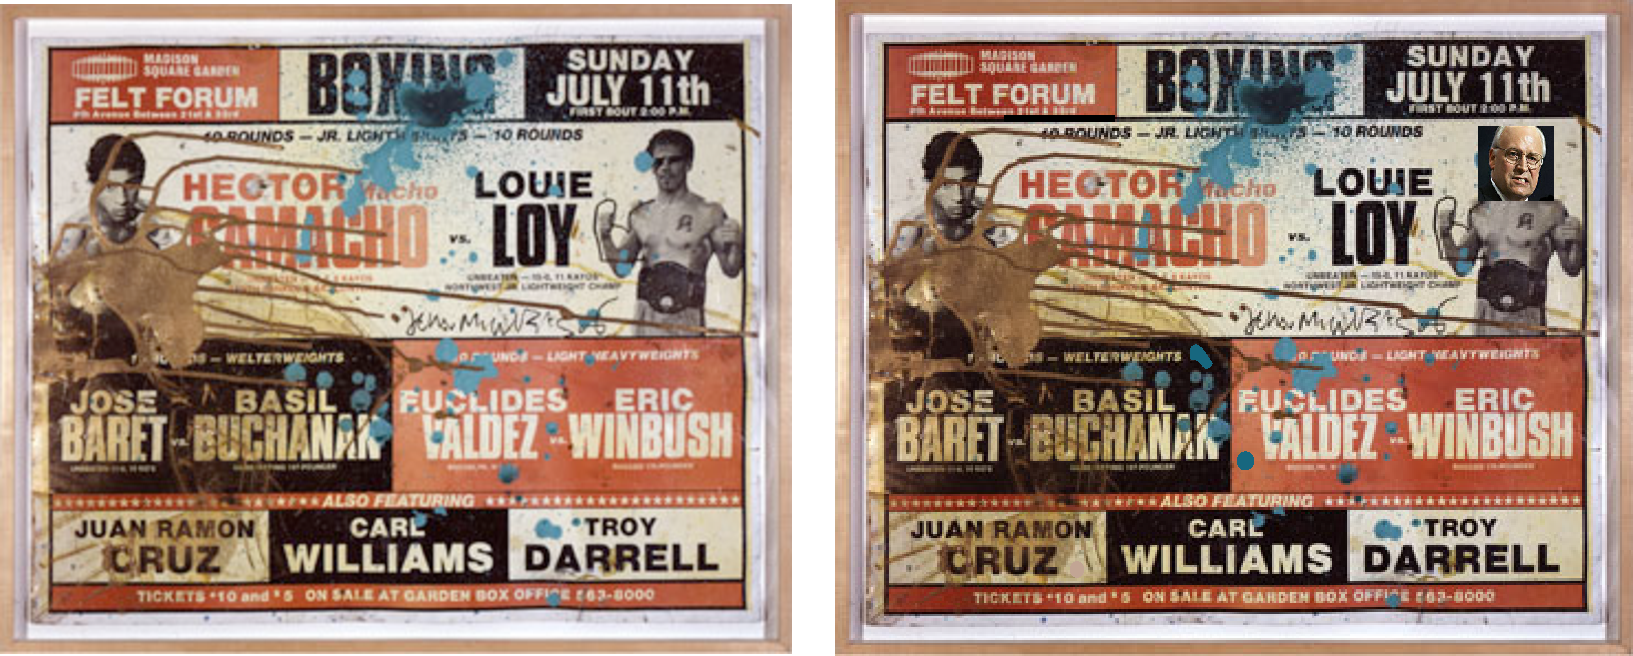
\includegraphics[height=1.8in]{../Art/RegistrationBasquiatDeWarp.pdf}
\newline
\newline
\newline
\| I ( x ) - J(\phi(x)) \|^2  + R(\phi( x)) 
\newline
\end{frame}

 \centeredlargetext{white}{black}{
\centering Enhanced user experience
%\newline
%
\includegraphics[height=1.8in]{../Art/ITKv4}
 }

 \centeredlargetext{white}{black}{
\centering Unified multi-core framework + parameter-estimation
%\newline
% 
\includegraphics[height=1.8in]{../Art/ITKv4}
 }


\begin{comment}
{

\begin{frame}
\frametitle{Image Registration Refactoring}
\Large
\begin{itemize}
\item Unify frameworks: local \& global 
\pause
\item New metrics and transform operations for vectors \&  tensors
\pause 
\item Composite Transform
\pause
\item Unbiased registration
\pause
\item Multi-threading 
\pause 
\item Automated parameter scaling
\end{itemize}
\end{frame}

\begin{frame}
\frametitle{Unified framework}
\Large
\begin{itemize}
\item Local \& global transforms treated the same in resampler
\item Both types available to (revised) optimizers
\item Revised metrics optimized for these operations
\item Tensors, vector, scalars treated transparently
\end{itemize}
\end{frame}
}
\end{comment}

 \centeredlargetext{white}{black}{
ITK v3 framework
\newline
\newline
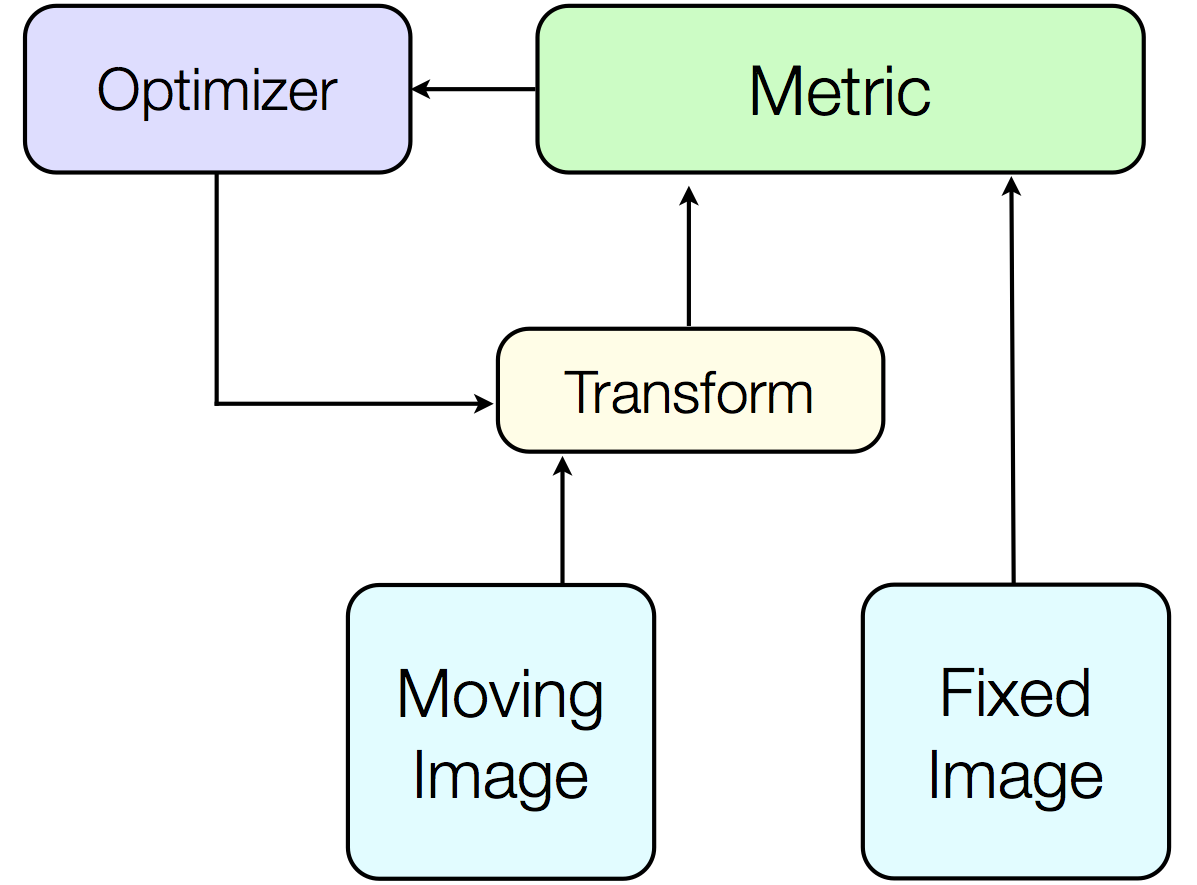
\includegraphics[height=2.2in]{../Art/itkv3reg}
 }

 \centeredlargetext{white}{black}{
ITK v4 framework
\newline
\newline
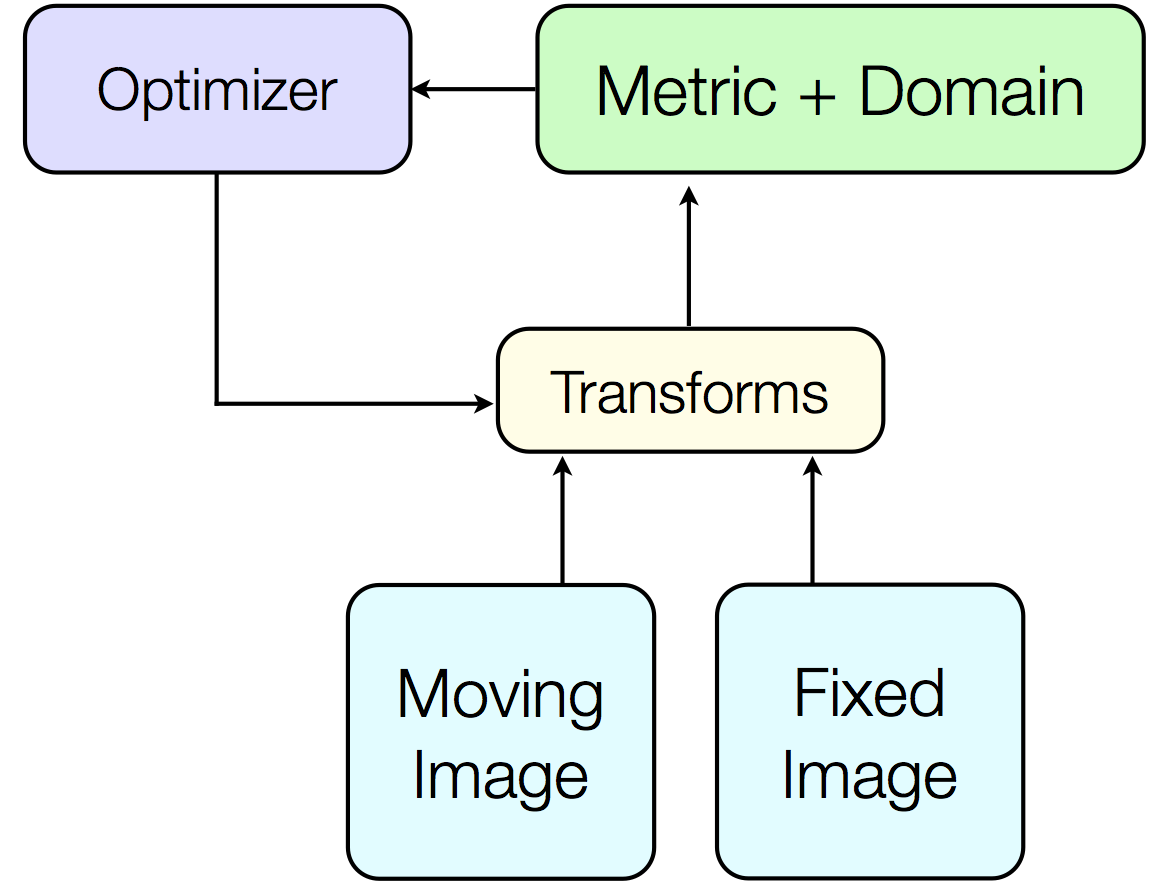
\includegraphics[height=2.2in]{../Art/itkv4reg}
 }

\begin{frame}
\frametitle{Composite transformations}
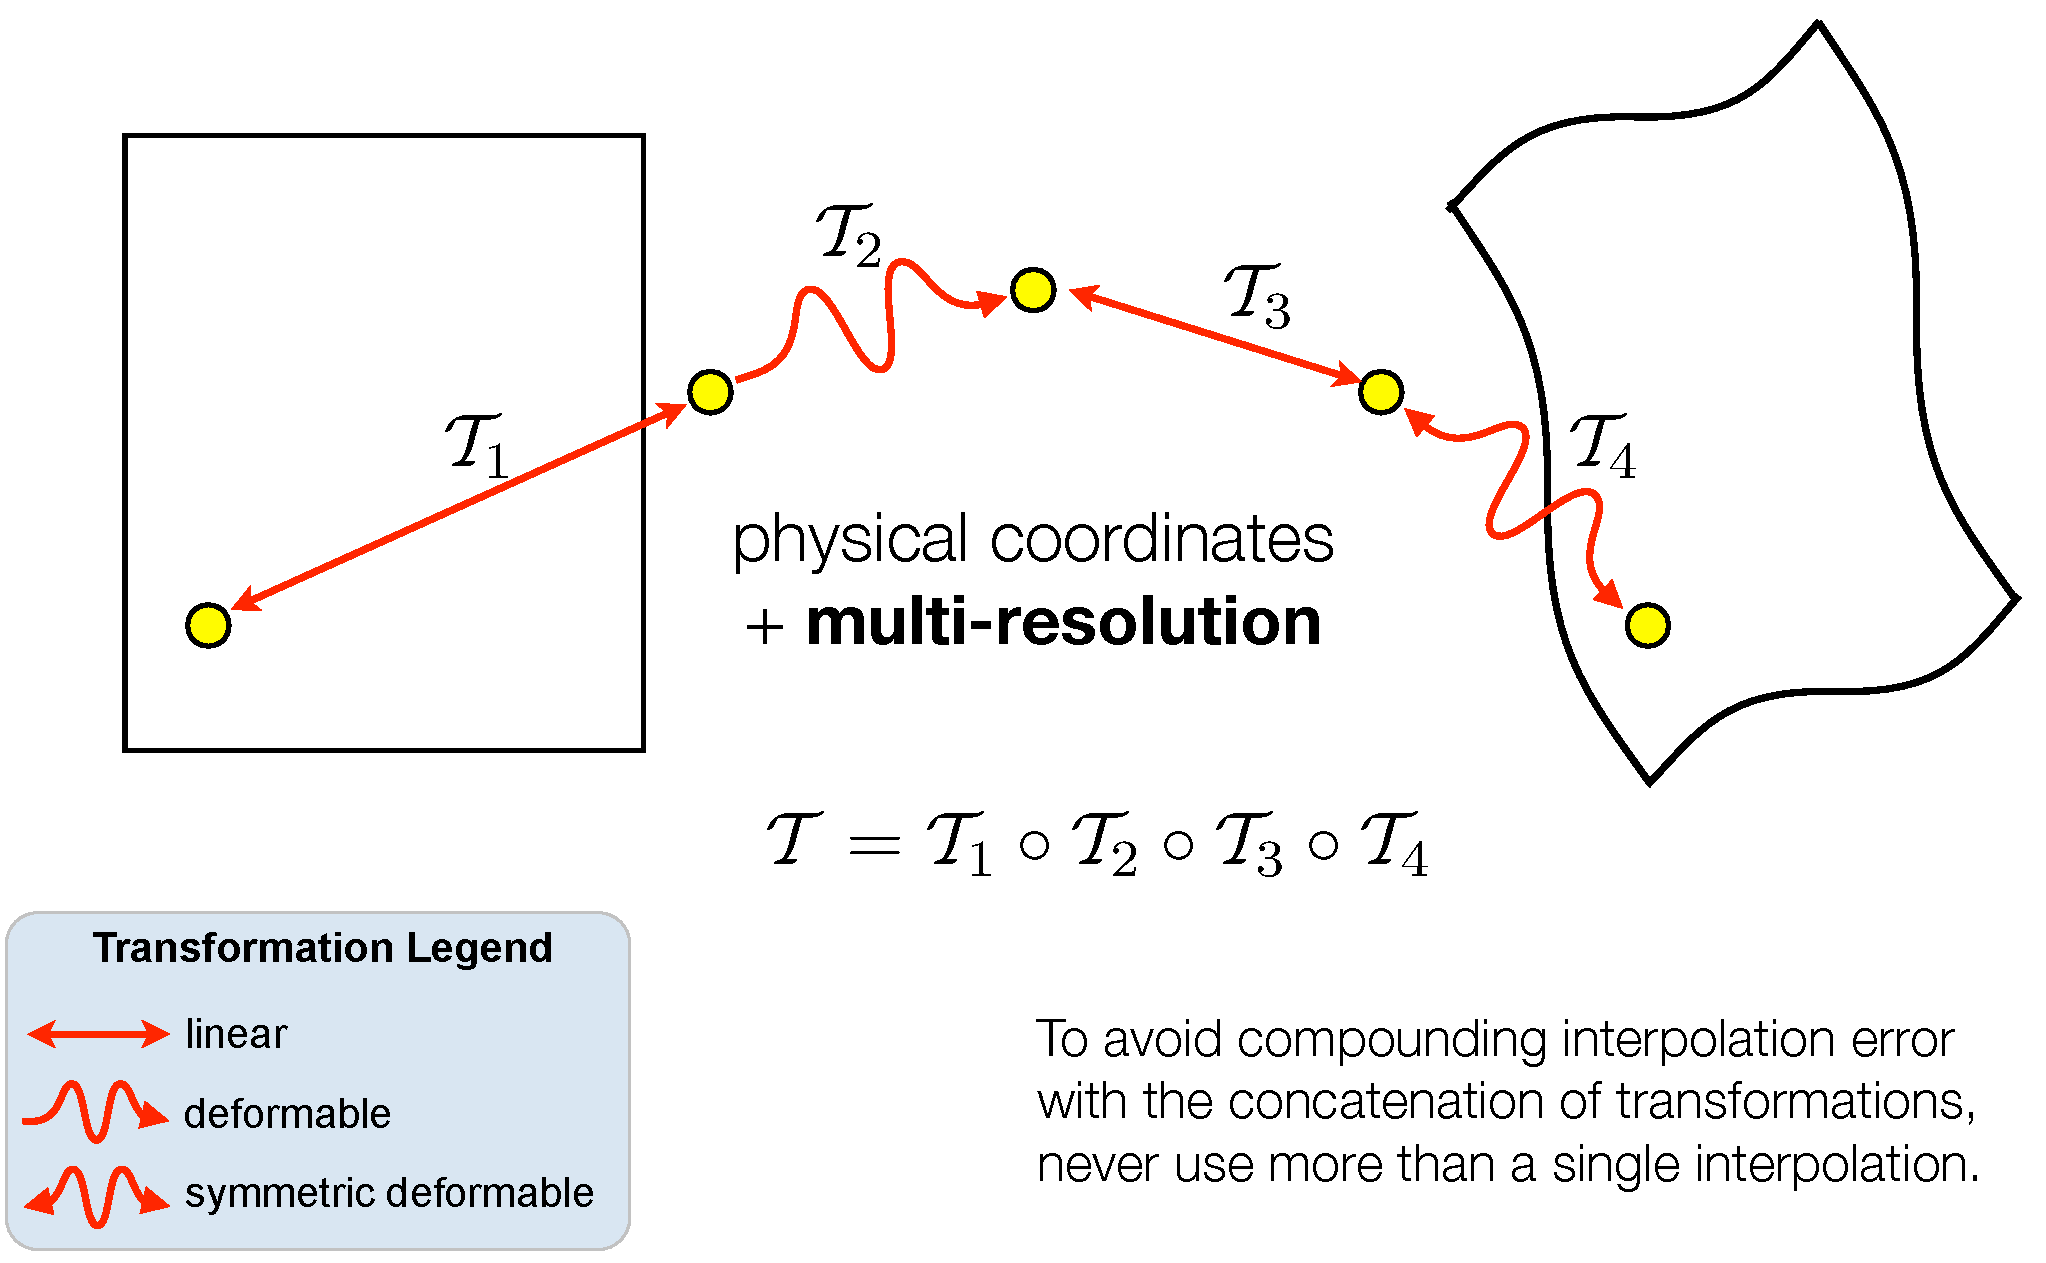
\includegraphics[height=2.5in]{../Art/composite}
\end{frame}

 \centeredlargetext{white}{black}{
\centering Example Registration
}

\begin{frame}
\frametitle{Compile external module}
\begin{itemize}
\item We link the external module
\lstlistingwithnumber{4}{5}{install_registration_code.cxx}
\item We recompile
\lstlistingwithnumber{6}{9}{install_registration_code.cxx}
\item Be sure to compile in Release mode for real applications!
\end{itemize}
\end{frame}


\begin{frame}
\frametitle{Image Registration Refactoring: Brain + N-hood CC}
\textcolor{red}{./bin/ITKRegistrationRefactoringTestDriver itkANTSNeighborhoodCorrelationImageToImageObjectRegistrationTest}\\
\textcolor{blue}{r16slice.jpg r64slice.jpg out.nii.gz  50 500 }\\
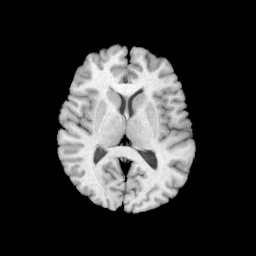
\includegraphics[height=2.2in]{../Art/r16slice.jpg}
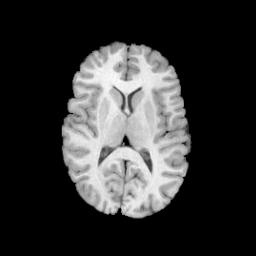
\includegraphics[height=2.2in]{../Art/r64slice.jpg}
\end{frame}

\begin{frame}
\frametitle{Image Registration Code: Brain + N-hood CC}
\begin{itemize}
\item Define the metric
\lstlistingwithnumber{171}{175}{itkANTSNeighborhoodCorrelationImageToImageObjectRegistrationTest.cxx}
\item Define the transforms
\lstlistingwithnumber{165}{168}{itkANTSNeighborhoodCorrelationImageToImageObjectRegistrationTest.cxx}
\lstlistingwithnumber{138}{141}{itkANTSNeighborhoodCorrelationImageToImageObjectRegistrationTest.cxx}
\item Resample the image
\lstlistingwithnumber{201}{202}{itkANTSNeighborhoodCorrelationImageToImageObjectRegistrationTest.cxx}
\end{itemize}

\end{frame}

\begin{frame}
\frametitle{Image Registration Refactoring: Composite Tx + MI}
\textcolor{red}{./bin/ITKRegistrationRefactoringTestDriver itkThevenazMutualInformationImageToImageObjectRegistrationTest }\\
\textcolor{blue}{face\_avg.jpg face\_c.jpg out.nii.gz  50 0.001 0.75 }\\
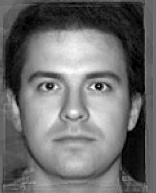
\includegraphics[height=2.2in]{../Art/face_avg.jpg}
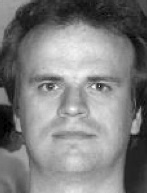
\includegraphics[height=2.2in]{../Art/face_c.jpg}
\end{frame}

\begin{frame}
\frametitle{Image Registration Result: Composite Tx + MI}
\textcolor{red}{./bin/ITKRegistrationRefactoringTestDriver itkThevenazMutualInformationImageToImageObjectRegistrationTest }\\
\textcolor{blue}{face\_avg.jpg face\_c.jpg out.nii.gz  50 0.001 0.75 }\\
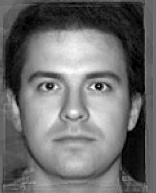
\includegraphics[height=2.2in]{../Art/face_avg.jpg}
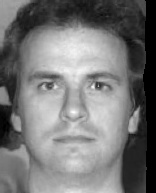
\includegraphics[height=2.2in]{../Art/face_c_to_face_avg.jpg}
\end{frame}

\begin{frame}
\frametitle{Image Registration Code: Composite Tx + MI}
\begin{itemize}
\item Define the metric
\lstlistingwithnumber{186}{189}{itkThevenazMutualInformationImageToImageObjectRegistrationTest.cxx}
\item Estimate scaling parameters for the affine transform
\lstlistingwithnumber{207}{210}{itkThevenazMutualInformationImageToImageObjectRegistrationTest.cxx}
\item Run the affine then add it to composite along with a new
  deformation transform
\lstlistingwithnumber{233}{238}{itkThevenazMutualInformationImageToImageObjectRegistrationTest.cxx}
\end{itemize}
\end{frame}

\begin{frame}
\frametitle{Image Registration Refactoring Example}
\textcolor{red}{./bin/ITKRegistrationRefactoringTestDriver itkThevenazMutualInformationImageToImageObjectRegistrationTest }\\
\textcolor{blue}{face\_avg.jpg face\_b.jpg out.nii.gz  50 0.001 0.75 }\\
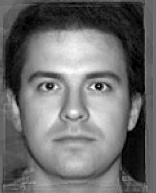
\includegraphics[height=2.2in]{../Art/face_avg.jpg}
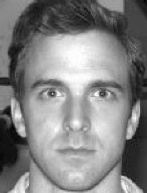
\includegraphics[height=2.2in]{../Art/face_b.jpg}
\end{frame}

\begin{frame}
\frametitle{Image Registration Refactoring Example}
\textcolor{red}{./bin/ITKRegistrationRefactoringTestDriver itkThevenazMutualInformationImageToImageObjectRegistrationTest }\\
\textcolor{blue}{face\_avg.jpg face\_b.jpg out.nii.gz  50 0.001 0.75 }\\
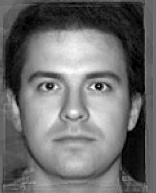
\includegraphics[height=2.2in]{../Art/face_avg.jpg}
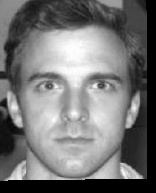
\includegraphics[height=2.2in]{../Art/face_b_to_face_avg_aff.jpg}
\end{frame}
\begin{frame}
\frametitle{Image Registration Refactoring Example}
\textcolor{red}{./bin/ITKRegistrationRefactoringTestDriver itkThevenazMutualInformationImageToImageObjectRegistrationTest }\\
\textcolor{blue}{face\_avg.jpg face\_b.jpg out.nii.gz  50 0.001 0.75 }\\
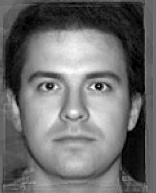
\includegraphics[height=2.2in]{../Art/face_avg.jpg}
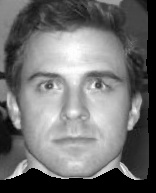
\includegraphics[height=2.2in]{../Art/face_b_to_face_avg.jpg}
\newline
25 seconds (1 thread) vs 16 seconds (2 threads) on Macbook Air.
\end{frame}

\begin{frame}
\frametitle{Image Registration Refactoring Example}
\textcolor{red}{./bin/ITKRegistrationRefactoringTestDriver itkThevenazMutualInformationImageToImageObjectRegistrationTest }\\
\textcolor{blue}{r16slice.jpg r64slice\_neg.jpg out.nii.gz  50 0.001 0.75 }\\
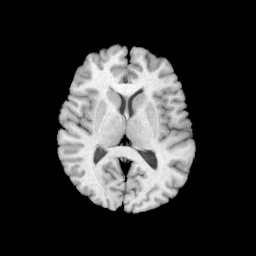
\includegraphics[height=2.2in]{../Art/r16slice.jpg}
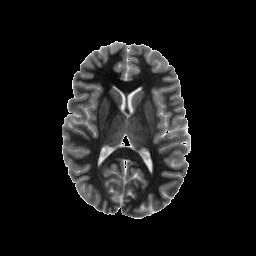
\includegraphics[height=2.2in]{../Art/r64slice_neg.jpg}
\end{frame}

\begin{frame}
\frametitle{Image Registration Refactoring Example}
\textcolor{red}{./bin/ITKRegistrationRefactoringTestDriver itkThevenazMutualInformationImageToImageObjectRegistrationTest }\\
\textcolor{blue}{r16slice.jpg r64slice\_neg.jpg out.nii.gz  50 0.001 0.75 }\\
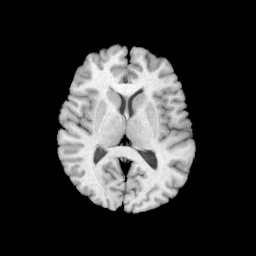
\includegraphics[height=2.2in]{../Art/r16slice.jpg}
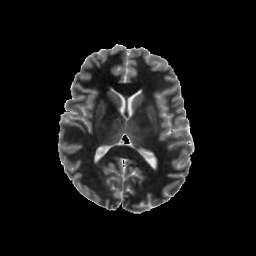
\includegraphics[height=2.2in]{../Art/r64slice_neg_to_16.jpg}
\end{frame}

\begin{frame}
\frametitle{New metrics}
\Large
\begin{itemize}
\item Metrics produce consistent results across threads.
\item Sparse and dense neighborhood correlation.
\item New mutual information implementation.
\item Point sets ---  euclidean, pse, Jensen-Havrda-Charvat-Tsallis (JHCT).
\item Tensor --- deviatoric and Euclidean.
\item Vector --- arbitrary length (non-geometric) and covariant.
\end{itemize}
\end{frame}

\begin{frame}
\frametitle{New transform models}
\Large
\begin{itemize}
\item As in ITKv3 $+$ some new ones + thread safety 
\item Displacement transforms
\item Updated bspline transforms
\item Poly-affine
\item Diffeomorphic (TBD)
\item Velocityfield --- needs optimizer
\item GPU Demons!!
\end{itemize}
\end{frame}

\begin{frame}
\frametitle{New optimizers}
\Large
\begin{itemize}
\item Multi-threaded update functions
\item Efficient use of parameters for high-dimensional transformations
\item Automated parameter adjustment via Quasi-Newton $+$ moving parameter estimation.
\end{itemize}
\end{frame}

\begin{frame}
\Large
\frametitle{Multi-threading}
\textcolor{red}{ ITK\_GLOBAL\_DEFAULT\_NUMBER\_OF\_THREADS=NT}\\
\textcolor{red}{export ITK\_GLOBAL\_DEFAULT\_NUMBER\_OF\_THREADS}
\newline
\newline
\textcolor{blue}{metric-$>$SetNumberOfThreads(2)}
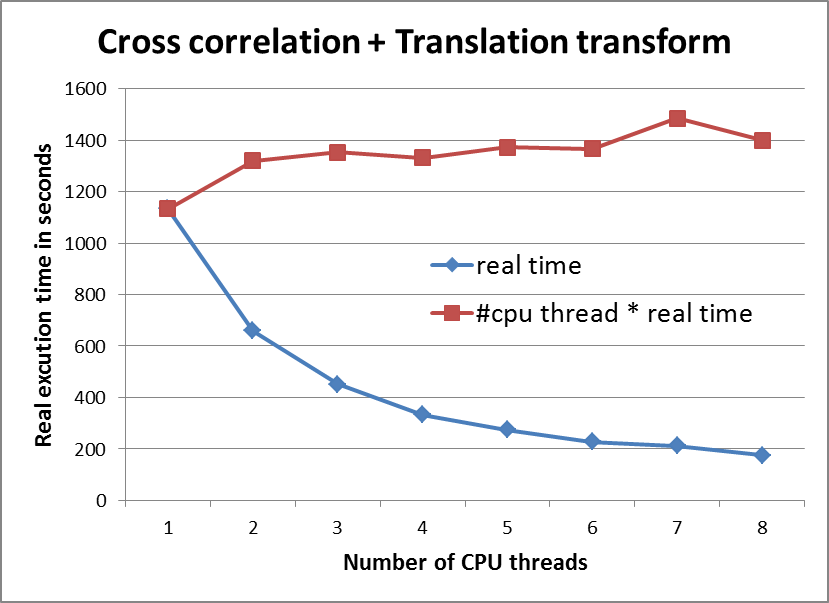
\includegraphics[height=1.5in]{../Art/cctran}~~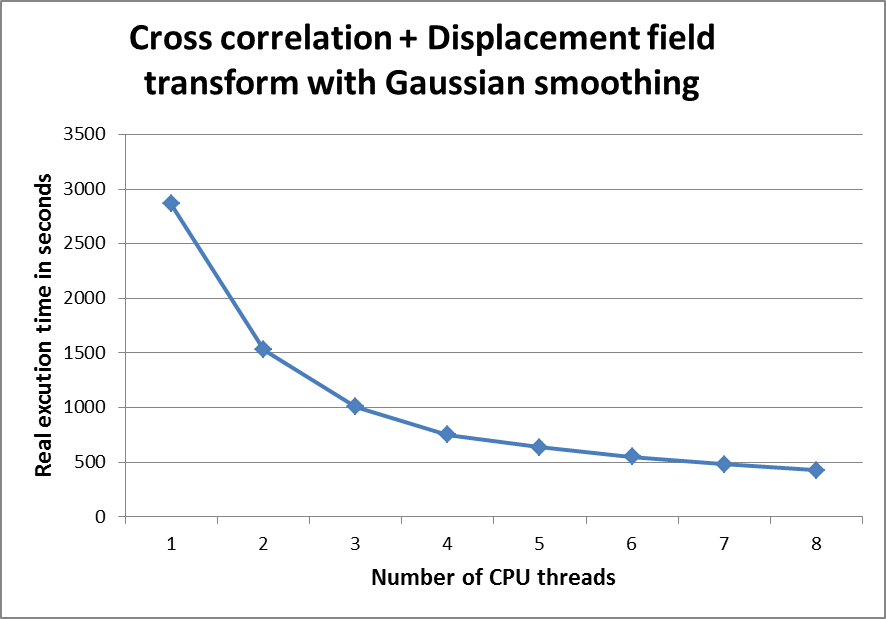
\includegraphics[height=1.5in]{../Art/ccfield}
\end{frame}

\begin{frame}
\Large
\frametitle{References relevant to ITKv4 development}
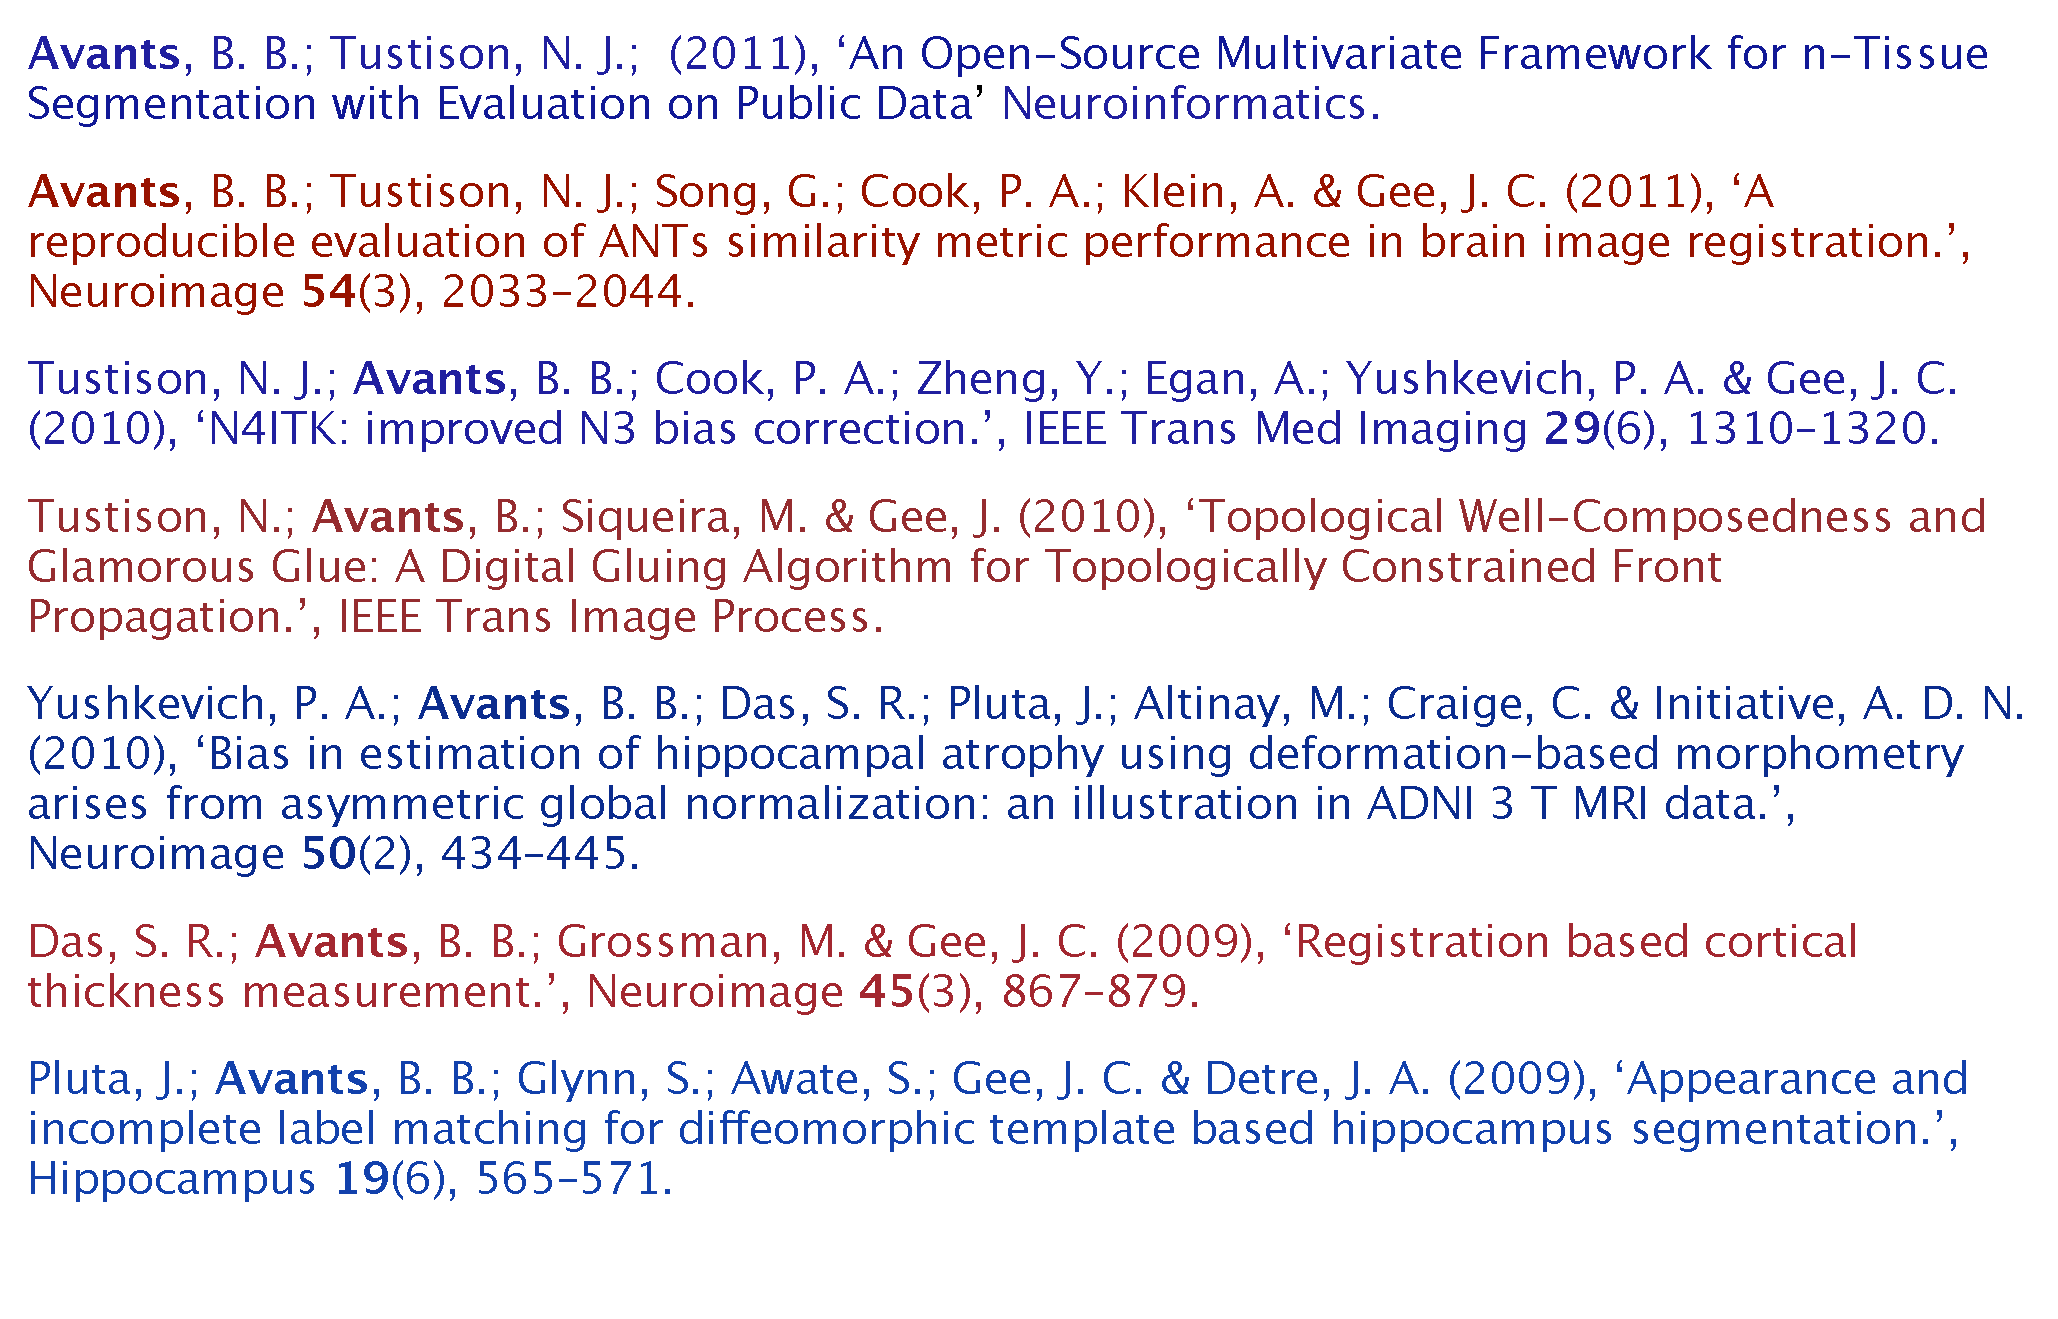
\includegraphics[height=3.2in]{../Art/registration_references}
\end{frame}

\begin{frame}
\Large
\frametitle{Recap \& Conclusion}
\begin{itemize}
\item Local \& global support transforms in same framework
\pause
\item Speed-up on multi-core machines for all high-dimensional metrics ($~N$-cores)
\pause
\item Multivariate and multi-component metrics coming!
\pause
\item Tensors, vector, scalars, landmarks, diffeomorphisms ... 
\pause
\item Evaluation will take some time and could use your help.
\pause
\item Looking forward to getting feedback on insight-users! 
\end{itemize}
\end{frame}
